% Options for packages loaded elsewhere
\PassOptionsToPackage{unicode}{hyperref}
\PassOptionsToPackage{hyphens}{url}
\PassOptionsToPackage{dvipsnames,svgnames,x11names}{xcolor}
%
\documentclass[
  11pt,
  ignorenonframetext,
]{beamer}
\usepackage{pgfpages}
\setbeamertemplate{caption}[numbered]
\setbeamertemplate{caption label separator}{: }
\setbeamercolor{caption name}{fg=normal text.fg}
\beamertemplatenavigationsymbolsempty
% Prevent slide breaks in the middle of a paragraph
\widowpenalties 1 10000
\raggedbottom
\setbeamertemplate{part page}{
  \centering
  \begin{beamercolorbox}[sep=16pt,center]{part title}
    \usebeamerfont{part title}\insertpart\par
  \end{beamercolorbox}
}
\setbeamertemplate{section page}{
  \centering
  \begin{beamercolorbox}[sep=12pt,center]{part title}
    \usebeamerfont{section title}\insertsection\par
  \end{beamercolorbox}
}
\setbeamertemplate{subsection page}{
  \centering
  \begin{beamercolorbox}[sep=8pt,center]{part title}
    \usebeamerfont{subsection title}\insertsubsection\par
  \end{beamercolorbox}
}
\AtBeginPart{
  \frame{\partpage}
}
\AtBeginSection{
  \ifbibliography
  \else
    \frame{\sectionpage}
  \fi
}
\AtBeginSubsection{
  \frame{\subsectionpage}
}
\usepackage{amsmath,amssymb}
\usepackage{lmodern}
\usepackage{setspace}
\usepackage{iftex}
\ifPDFTeX
  \usepackage[T1]{fontenc}
  \usepackage[utf8]{inputenc}
  \usepackage{textcomp} % provide euro and other symbols
\else % if luatex or xetex
  \usepackage{unicode-math}
  \defaultfontfeatures{Scale=MatchLowercase}
  \defaultfontfeatures[\rmfamily]{Ligatures=TeX,Scale=1}
\fi
% Use upquote if available, for straight quotes in verbatim environments
\IfFileExists{upquote.sty}{\usepackage{upquote}}{}
\IfFileExists{microtype.sty}{% use microtype if available
  \usepackage[]{microtype}
  \UseMicrotypeSet[protrusion]{basicmath} % disable protrusion for tt fonts
}{}
\makeatletter
\@ifundefined{KOMAClassName}{% if non-KOMA class
  \IfFileExists{parskip.sty}{%
    \usepackage{parskip}
  }{% else
    \setlength{\parindent}{0pt}
    \setlength{\parskip}{6pt plus 2pt minus 1pt}}
}{% if KOMA class
  \KOMAoptions{parskip=half}}
\makeatother
\usepackage{xcolor}
\geometry{left = 1cm, right = 0.5cm, top = 0.5cm, bottom = 0.5cm}
\newif\ifbibliography
\usepackage{graphicx}
\makeatletter
\def\maxwidth{\ifdim\Gin@nat@width>\linewidth\linewidth\else\Gin@nat@width\fi}
\def\maxheight{\ifdim\Gin@nat@height>\textheight\textheight\else\Gin@nat@height\fi}
\makeatother
% Scale images if necessary, so that they will not overflow the page
% margins by default, and it is still possible to overwrite the defaults
% using explicit options in \includegraphics[width, height, ...]{}
\setkeys{Gin}{width=\maxwidth,height=\maxheight,keepaspectratio}
% Set default figure placement to htbp
\makeatletter
\def\fps@figure{htbp}
\makeatother
\setlength{\emergencystretch}{3em} % prevent overfull lines
\providecommand{\tightlist}{%
  \setlength{\itemsep}{0pt}\setlength{\parskip}{0pt}}
\setcounter{secnumdepth}{-\maxdimen} % remove section numbering
\titlegraphic{
\includegraphics[scale=0.05]{pictures/GlaLogo.pdf}}
\usepackage{float}
\usepackage{booktabs}
\usepackage{array}
\usepackage{longtable}
\setbeamertemplate{itemize item}{$\diamond$}
\setbeamertemplate{itemize subitem}{\scriptsize$\diamond$}
\setbeamertemplate{itemize subsubitem}{\scriptsize$\gg$}
\definecolor{blue}{RGB}{0,114,178}
\definecolor{red}{RGB}{213,94,0}
\definecolor{yellow}{RGB}{240,228,66}
\definecolor{green}{RGB}{0,158,115}
\ifLuaTeX
  \usepackage{selnolig}  % disable illegal ligatures
\fi
\IfFileExists{bookmark.sty}{\usepackage{bookmark}}{\usepackage{hyperref}}
\IfFileExists{xurl.sty}{\usepackage{xurl}}{} % add URL line breaks if available
\urlstyle{same} % disable monospaced font for URLs
\hypersetup{
  pdftitle={Introductory Statistics for Economics},
  pdfauthor={Duong Trinh},
  colorlinks=true,
  linkcolor={blue},
  filecolor={Maroon},
  citecolor={Blue},
  urlcolor={Blue},
  pdfcreator={LaTeX via pandoc}}

\title{Introductory Statistics for Economics}
\subtitle{ECON1013: TUTORIAL 2}
\author{Duong Trinh}
\date{Spring 2024}
\institute{University of Glasgow}

\begin{document}
\frame{\titlepage}

\setstretch{1.5}
\begin{frame}{Intro}
\protect\hypertarget{intro}{}
\begin{itemize}
\tightlist
\item
  Duong Trinh

  \begin{itemize}
  \tightlist
  \item
    PhD Student in Economics (Bayesian Microeconometrics)
  \item
    Email: \underline{Duong.Trinh@glasgow.ac.uk}
  \end{itemize}
\end{itemize}

\vspace{3mm}

\begin{itemize}
\tightlist
\item
  ECON1013-TU04

  \begin{itemize}
  \tightlist
  \item
    Monday 12-1 pm
  \item
    4 sessions (22-Jan, 5-Feb, 19-Feb, 4-March)
  \end{itemize}
\item
  ECON1013-TU05

  \begin{itemize}
  \tightlist
  \item
    Tuesday 12-1 pm
  \item
    4 sessions (23-Jan, 6-Feb, 20-Feb, 5-March)
  \end{itemize}
\item
  ECON1013-TU07

  \begin{itemize}
  \tightlist
  \item
    Tuesday 2-3 pm
  \item
    4 sessions (23-Jan, 6-Feb, 20-Feb, 5-March)
  \end{itemize}
\end{itemize}
\end{frame}

\begin{frame}{Record Attendance}
\protect\hypertarget{record-attendance}{}
\end{frame}

\begin{frame}{Exercise 1}
\protect\hypertarget{exercise-1}{}
\begin{columns}[T]
\begin{column}{.7\textwidth}
\begin{itemize}
\tightlist
\item
  Let \(X\) be the amount of exported grain next month (in tonnes) of a
  grain exporting company.
\end{itemize}

\vspace{3mm}

\begin{itemize}
\tightlist
\item
  Based on previous exporting records, the company estimates that the
  exporting probabilities and amounts.
\end{itemize}
\end{column}

\begin{column}{0.48\textwidth}
\begin{table}
\centering
\begin{tabular}{cc}
\hline
x & P(x) \tabularnewline
\hline
100 & 0.05 \tabularnewline
150 & 0.20 \tabularnewline
200 & 0.50 \tabularnewline
250 & 0.20 \tabularnewline
300 & 0.05 \tabularnewline
\hline
\end{tabular}
\end{table}
\end{column}
\end{columns}
\end{frame}

\begin{frame}{Exercise 1}
\protect\hypertarget{exercise-1-1}{}
\begin{enumerate}
[(a)]
\tightlist
\item
  What is the probability that the company does not export more than 250
  tonnes?
\end{enumerate}

\quad\quad \(\color{blue}{P(X \leq 250) = ?}\)

\begin{enumerate}
[(a)]
\setcounter{enumi}{1}
\tightlist
\item
  What is the expected amount of tonnes that the company will export?
\end{enumerate}

\quad\quad \(\color{blue}{E[X] = ?}\)

\begin{enumerate}
[(a)]
\setcounter{enumi}{2}
\tightlist
\item
  What is the standard deviation?
\end{enumerate}

\quad\quad \(\color{blue}{\sqrt{Var[X]} = ?}\)
\end{frame}

\begin{frame}{(a) What is the probability that the company doesn't
export more than 250 tonnes?}
\protect\hypertarget{a-what-is-the-probability-that-the-company-doesnt-export-more-than-250-tonnes}{}
\begin{columns}[T]
\begin{column}{.7\textwidth}
\begin{itemize}
\tightlist
\item
  From the cumulative probability distribution we see that the
  probability that the company does not export more than \(250\) tonnes
  is \[
  P(X\leq 250) = F(250) = 0.95
  \]
\end{itemize}
\end{column}

\begin{column}{0.48\textwidth}
\begin{table}
\centering
\begin{tabular}{ccc}
\hline
x & P(x) & F(x) \tabularnewline
\hline
100 & 0.05 & 0.05 \tabularnewline
150 & 0.20 & 0.25\tabularnewline
200 & 0.50 & 0.75\tabularnewline
250 & 0.20 & 0.95\tabularnewline
300 & 0.05 & 1.00\tabularnewline
\hline
\end{tabular}
\end{table}
\end{column}
\end{columns}
\end{frame}

\begin{frame}{(b) What is the expected amount of tonnes that the company
will export?}
\protect\hypertarget{b-what-is-the-expected-amount-of-tonnes-that-the-company-will-export}{}
\small

\[
\begin{aligned}
E[X] = \mu &= \sum_x xP(x)\\
&= 100\times 0.05 + 150 \times 0.20 + 200 \times 0.50 + 250\times 0.20 + 300\times 0.05\\ 
&=200
\end{aligned}
\]
\end{frame}

\begin{frame}{(c) What is the standard deviation?}
\protect\hypertarget{c-what-is-the-standard-deviation}{}
\small

\[
\begin{aligned}
\sigma &= \sqrt{\sum_x (x-\mu)^2 P(x)}\\
&= \sqrt{(100-200)^2 \times 0.05 + (150-200)^2 \times 0.20 + \ldots + (300-200)^2\times 0.05}\\
&= \sqrt{2000}\\
&\approx 44.72
\end{aligned}
\]
\end{frame}

\begin{frame}{Exercise 1}
\protect\hypertarget{exercise-1-2}{}
\begin{columns}[T]
\begin{column}{.7\textwidth}
\begin{itemize}
\tightlist
\item
  Let \(Y\) be the amount of exported salt (in tonnes) next month of the
  company.
\end{itemize}

\vspace{5mm}

\begin{itemize}
\tightlist
\item
  The contracts for salt allow for salt being sold in much smaller
  quantities, making it a continuous random variable. \[
  Y \sim \mathcal{N}(120,30^2)
  \]
\end{itemize}
\end{column}

\begin{column}{0.48\textwidth}
\small

\[
\mu_Y = 120; \quad \sigma_Y = 30
\]

\begin{center}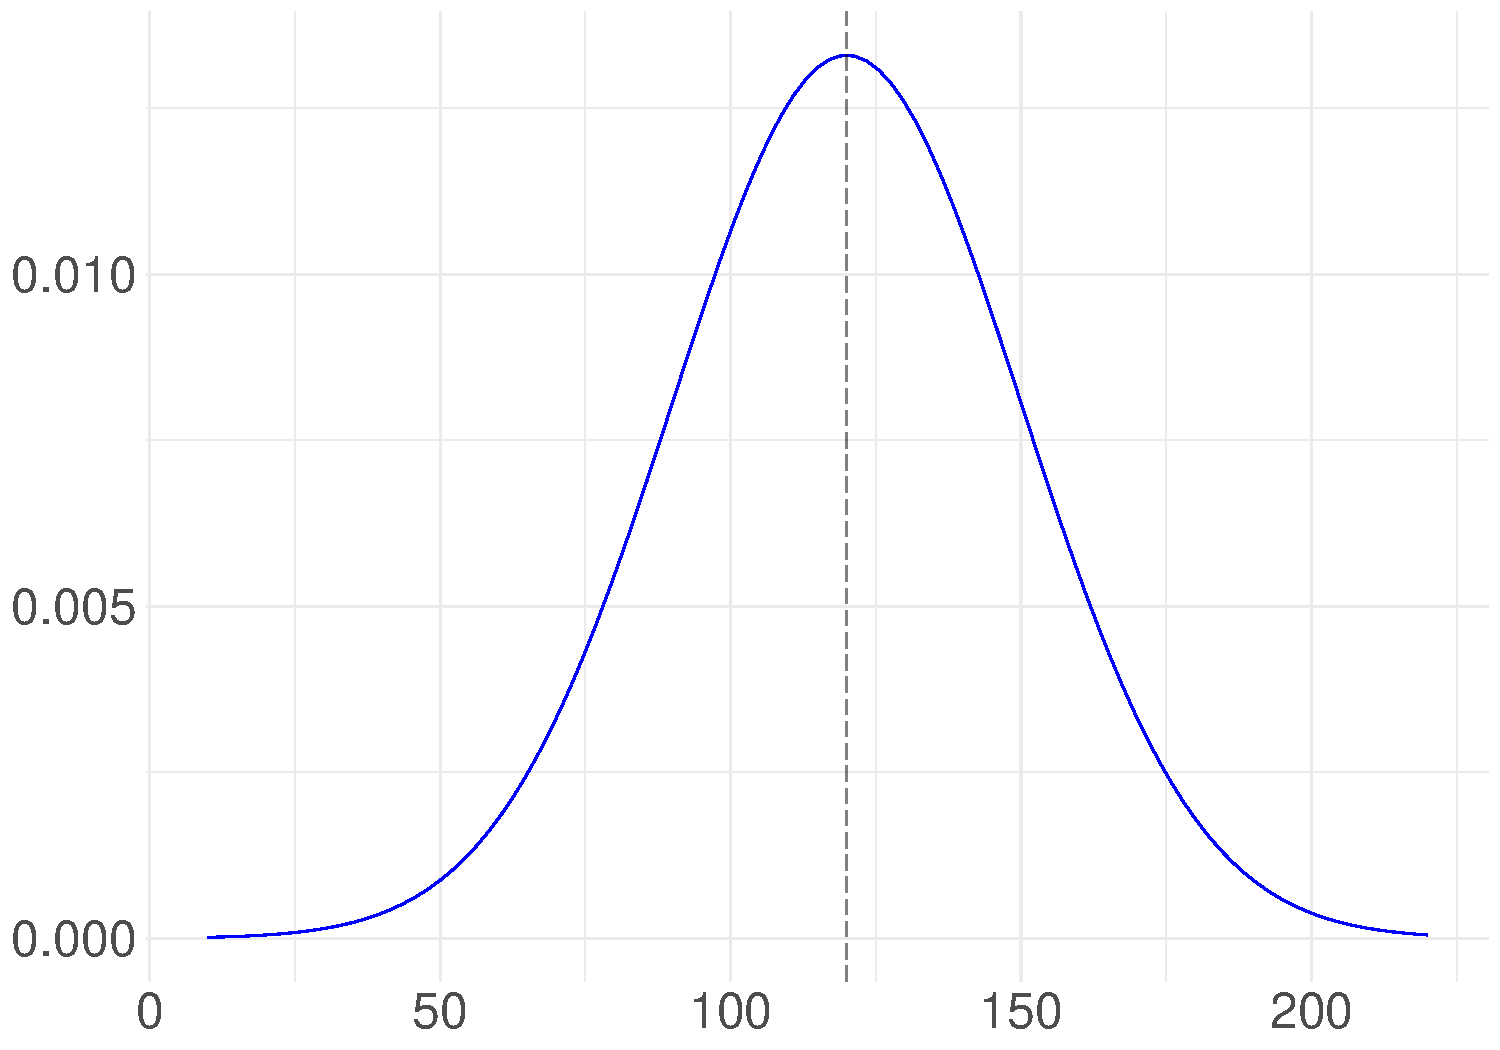
\includegraphics[width=0.8\linewidth]{ECON1013_Tutorial2_files/figure-beamer/unnamed-chunk-4-1} \end{center}
\end{column}
\end{columns}
\end{frame}

\begin{frame}{Exercise 1}
\protect\hypertarget{exercise-1-3}{}
\begin{enumerate}
[(a)]
\setcounter{enumi}{3}
\tightlist
\item
  What is the probability that the amount of exported salt next month
  will not be bigger than \(160\) tonnes?
\end{enumerate}

\quad\quad \(\color{blue}{P(Y \leq 160) = ?}\)

\begin{enumerate}
[(a)]
\setcounter{enumi}{4}
\tightlist
\item
  What is the probability that the amount of exported salt next month
  will be between \(80\) and \(160\) tonnes?
\end{enumerate}

\quad\quad \(\color{blue}{P(80 \leq Y \leq 160) = ?}\)
\end{frame}

\begin{frame}{(d) What is the probability that the amount of exported
salt next month will not be bigger than \(160\) tonnes?}
\protect\hypertarget{d-what-is-the-probability-that-the-amount-of-exported-salt-next-month-will-not-be-bigger-than-160-tonnes}{}
\normalsize

S1. Transform \(Y\) into the standard normal random variable \(Z\)
\small \[
Z = \frac{Y - \mu}{\sigma} = \frac{Y - 120}{30}; \quad Z \sim \mathcal{N}(0,1^2)
\]

\normalsize

S2. Rewrite the probability by transforming \(160\) tonnes to \(Z\)
units \small \[
P(Y \leq 160) = P\left(\frac{Y - 120}{30} \leq \frac{160 - 120}{30}\right) \approx P\left(Z \leq 1.33\right)
\]

\normalsize

S3. Looked up from a standard normal distribution statistical table
\small \[
P\left(Z \leq 1.33\right) = F(1.33) \approx 0.908
\]
\end{frame}

\begin{frame}{(d) What is the probability that the amount of exported
salt next month will not be bigger than \(160\) tonnes?}
\protect\hypertarget{d-what-is-the-probability-that-the-amount-of-exported-salt-next-month-will-not-be-bigger-than-160-tonnes-1}{}
\begin{center}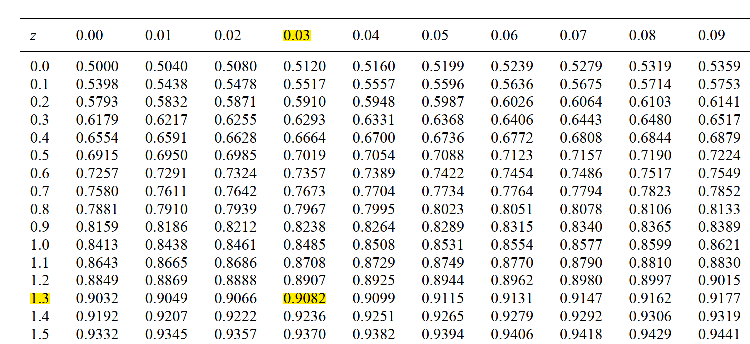
\includegraphics[width=0.9\linewidth]{pictures/Zat1.33} \end{center}
\end{frame}

\begin{frame}{(e) What is the probability that the amount of exported
salt next month will be between \(80\) and \(160\) tonnes?}
\protect\hypertarget{e-what-is-the-probability-that-the-amount-of-exported-salt-next-month-will-be-between-80-and-160-tonnes}{}
\normalsize

S1. Transform \(Y\) into the standard normal random variable \(Z\)
\small \[
Z = \frac{Y - \mu}{\sigma} = \frac{Y - 120}{30}
\] \normalsize S2. Rewrite the probability \small \[
\begin{aligned}
P(80 \leq Y \leq 160) &= P\left(\frac{80 - 120}{30} \leq \frac{Y - 120}{30} \leq \frac{160 - 120}{30}\right)\\
&\approx P\left(-1.33 \leq Z \leq 1.33\right)\\
&= 1 - [ P\left(Z \geq 1.33\right) + P\left(Z \leq -1.33\right)]\\
&= 1- 2P\left(Z \geq 1.33\right)\\
&= 1 -2[1-P\left(Z \leq 1.33\right)]\\
&= 2F(1.33)\\
& \approx 2 \times 0.908 -1 = 0.816
\end{aligned}
\]
\end{frame}

\begin{frame}{(e) What is the probability that the amount of exported
salt next month will be between \(80\) and \(160\) tonnes?}
\protect\hypertarget{e-what-is-the-probability-that-the-amount-of-exported-salt-next-month-will-be-between-80-and-160-tonnes-1}{}
\begin{center}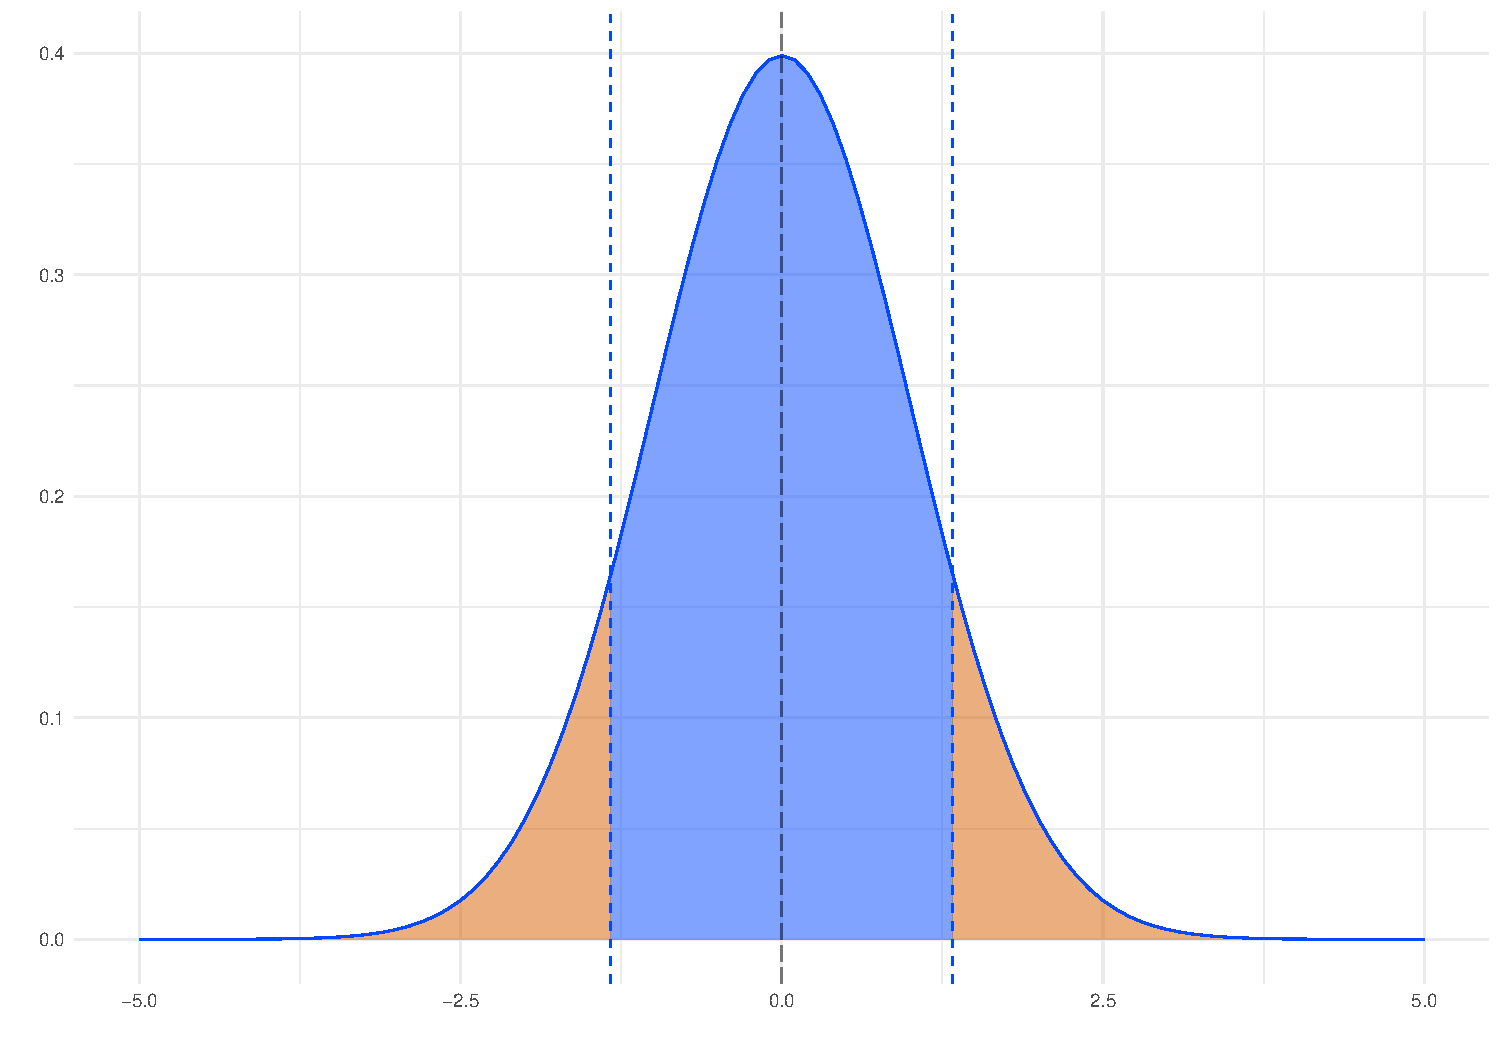
\includegraphics[width=0.8\linewidth]{ECON1013_Tutorial2_files/figure-beamer/unnamed-chunk-6-1} \end{center}
\end{frame}

\begin{frame}{(e) What is the probability that the amount of exported
salt next month will be between \(80\) and \(160\) tonnes?}
\protect\hypertarget{e-what-is-the-probability-that-the-amount-of-exported-salt-next-month-will-be-between-80-and-160-tonnes-2}{}
\begin{center}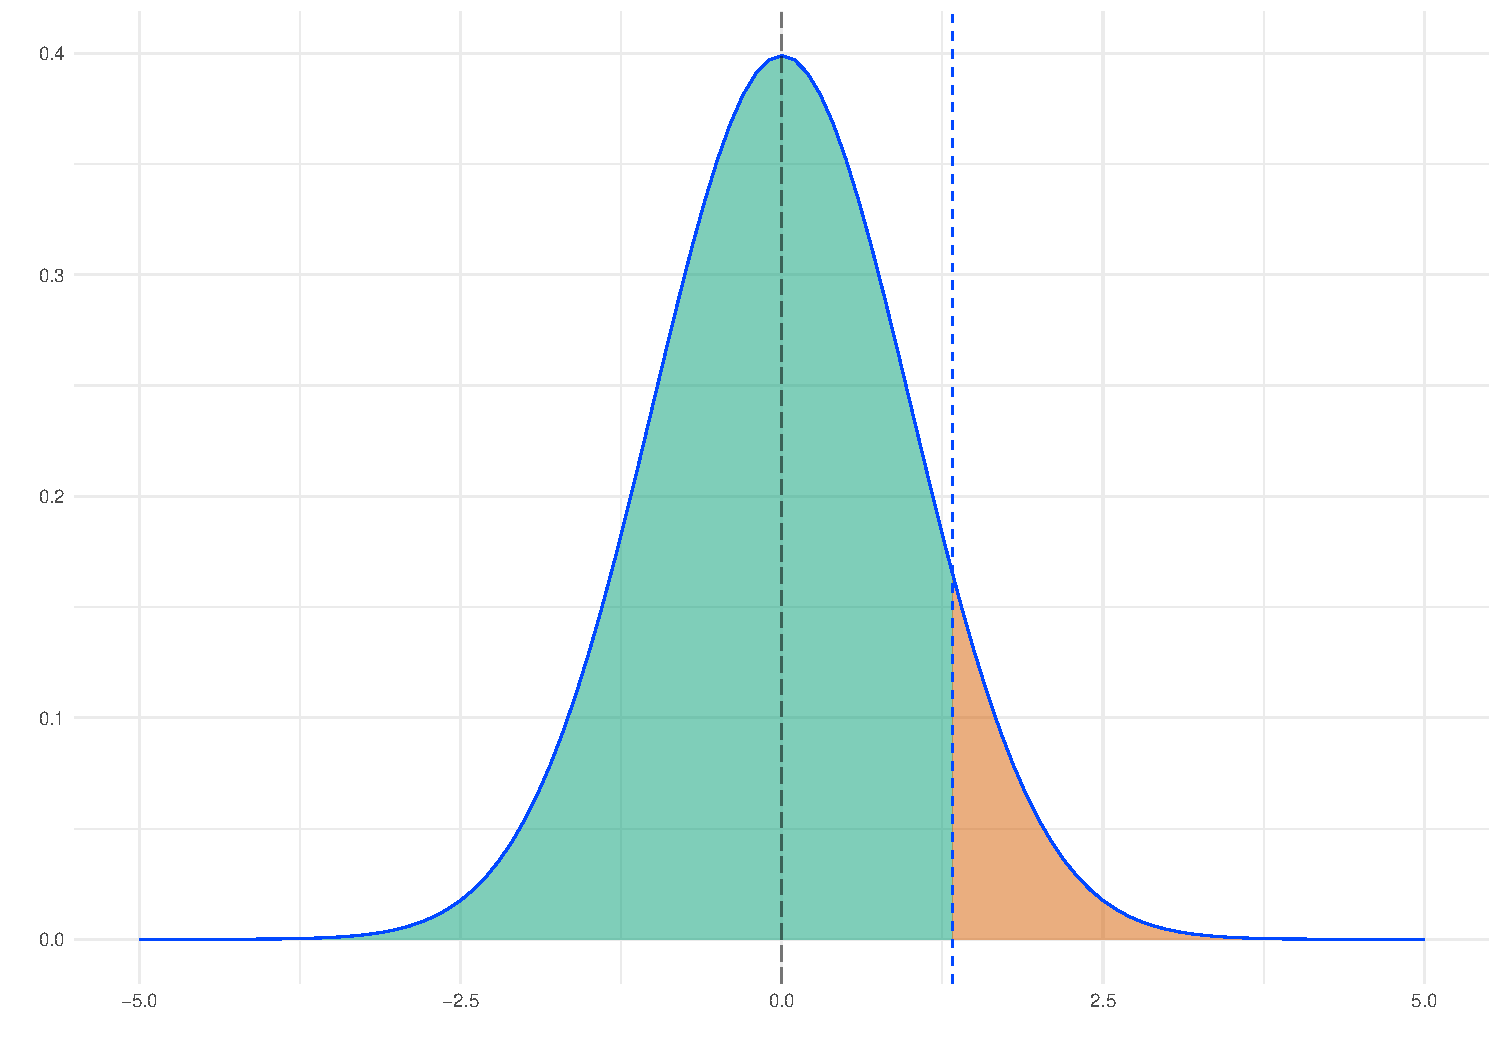
\includegraphics[width=0.8\linewidth]{ECON1013_Tutorial2_files/figure-beamer/unnamed-chunk-7-1} \end{center}
\end{frame}

\begin{frame}{Exercise 2}
\protect\hypertarget{exercise-2}{}
\begin{itemize}
\item
  A population consists of all first-year primary school students in a
  specific neighborhood \((N = 500)\).
\item
  Administrative data on the number of years spent in nursery of the
  full population of students:

  \begin{itemize}
  \tightlist
  \item
    Population mean: \(\mu = 3\)
  \item
    Population standard deviation: \(\sigma = 1.6\)
  \end{itemize}
\item
  Pick a random sample of \(n = 47\) students.

  \begin{itemize}
  \tightlist
  \item
    Denote by \(\bar{X}\) the random variable ``sample mean'' and by
    \(\bar{x}\) its realization.
  \end{itemize}
\end{itemize}
\end{frame}

\begin{frame}{Exercise 2}
\protect\hypertarget{exercise-2-1}{}
\begin{enumerate}
[(a)]
\item
  Explain what do we mean by ``\emph{the sampling distribution of the
  sample mean} (\(\bar{X}\))''?
\item
  Using your knowledge about sampling (without making any calculations),
  characterize the sampling distribution of \(\bar{X}\).
\item
  Calculate the \emph{mean} and \emph{standard deviation} of the
  sampling distribution.
\item
  What values of \(\bar{X}\) are likely? Would, for example, a sample
  mean \(\bar{x} = 3.5\) be likely or unlikely?
\end{enumerate}
\end{frame}

\begin{frame}{(a) Explain what do we mean by ``\emph{the sampling
distribution of the sample mean} (\(\bar{X}\))''?}
\protect\hypertarget{a-explain-what-do-we-mean-by-the-sampling-distribution-of-the-sample-mean-barx}{}
\begin{itemize}
\item
  It tells us how sample means are distributed across samples
\item
  It tells us how likely are different possible values of \(\bar{x}\)
  given the population parameters and the sample size.
\end{itemize}
\end{frame}

\begin{frame}{(b) Characterize the sampling distribution of
\(\bar{X}\).}
\protect\hypertarget{b-characterize-the-sampling-distribution-of-barx.}{}
\textcolor{red}{Central Limit Theorem}

\begin{itemize}
\item
  In word: the sampling distribution of the sample mean is approximately
  normal when the sample size is large enough.
\item
  In math:
\end{itemize}

\[
  \bar{X} \sim \mathcal{N}\left(\mu_{\bar X},\sigma^2_{\bar X}\right)
  \]

Sample size \(n = 47\) is sufficiently large (i.e.~\(\geq 30\)) to have
an approximately normally distributed sampling distribution of the
sample mean. This is true even if the population distribution of \(X\)
is not normal.
\end{frame}

\begin{frame}{}
\protect\hypertarget{section}{}
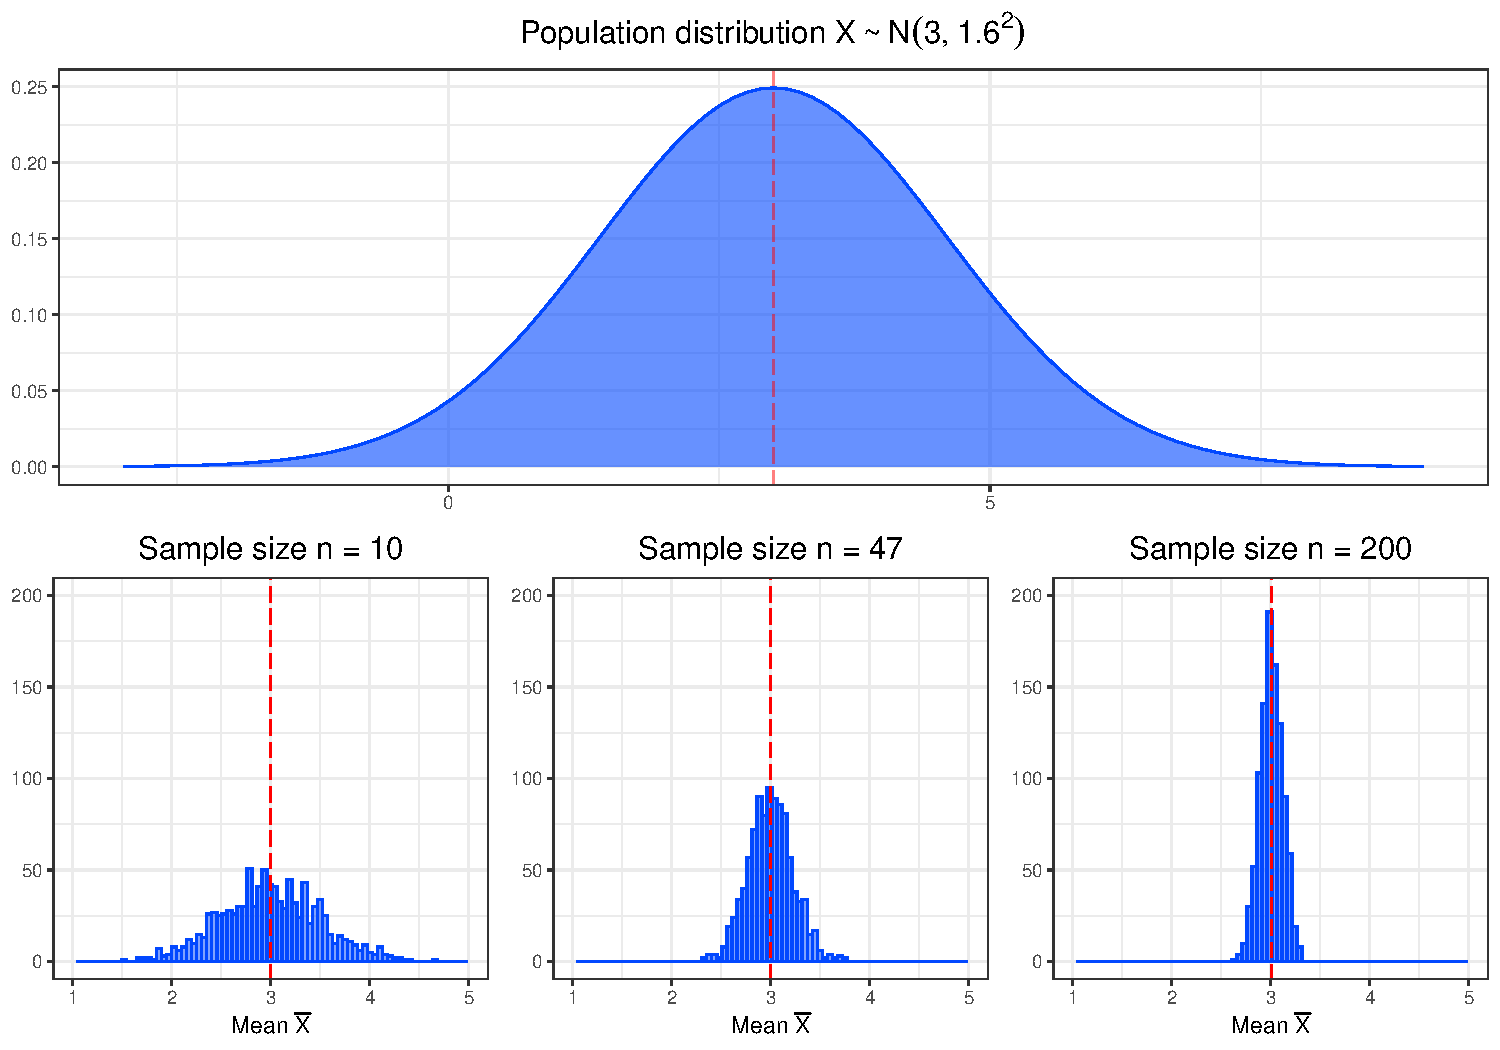
\includegraphics{ECON1013_Tutorial2_files/figure-beamer/unnamed-chunk-9-1.pdf}
\end{frame}

\begin{frame}{}
\protect\hypertarget{section-1}{}
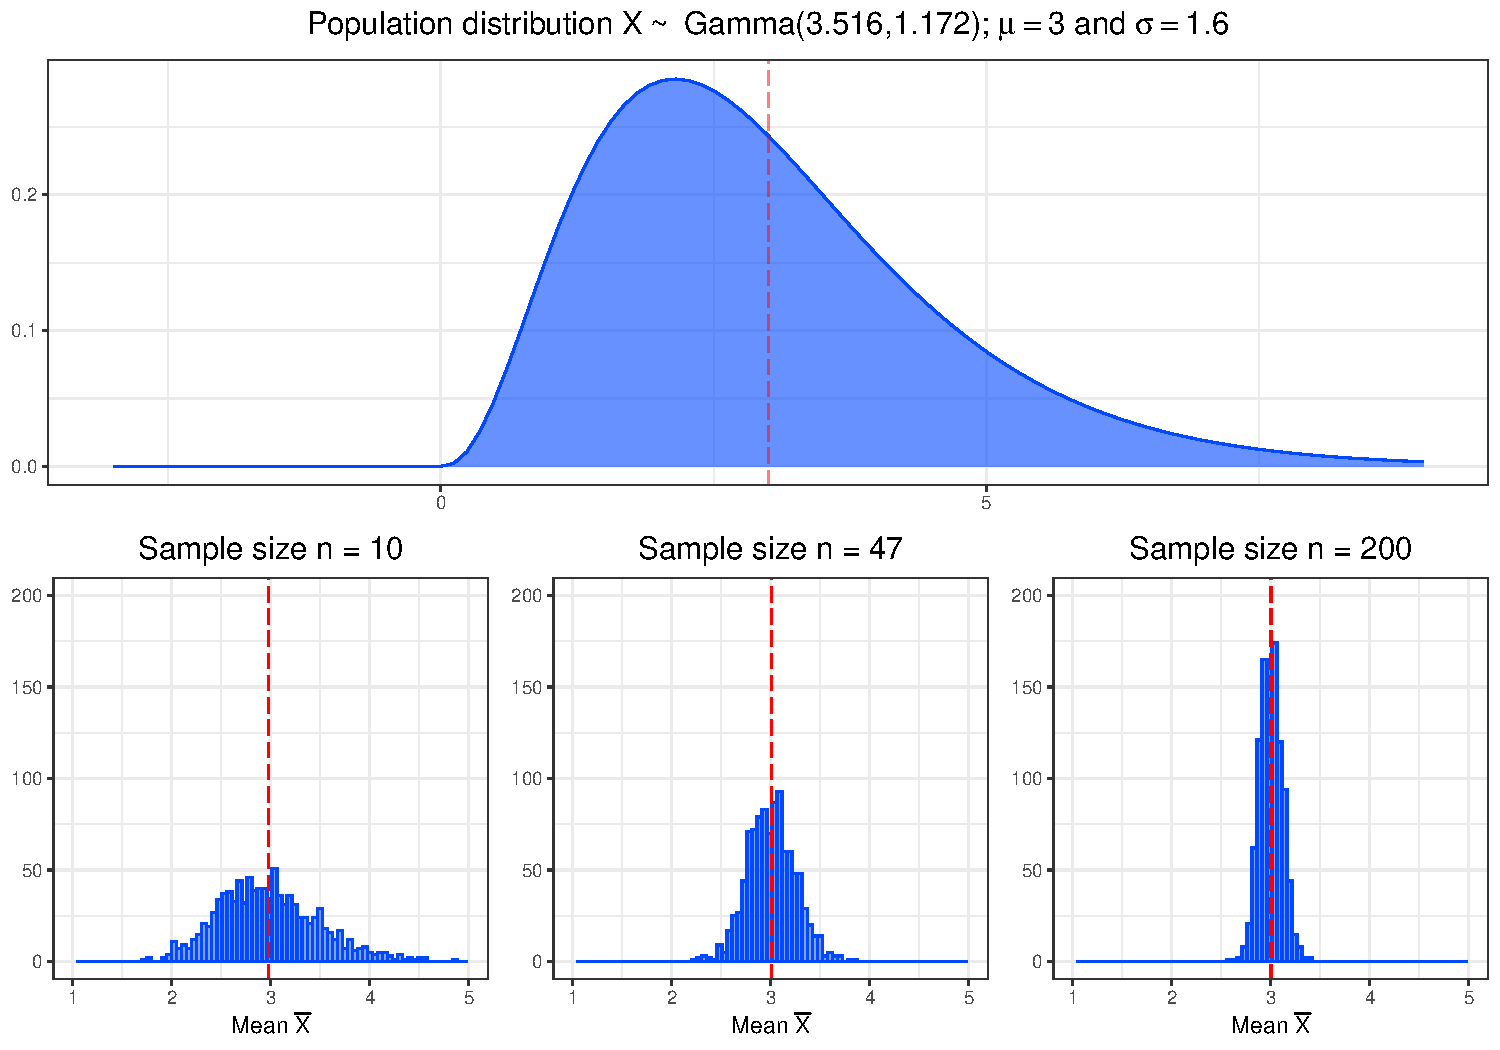
\includegraphics{ECON1013_Tutorial2_files/figure-beamer/unnamed-chunk-10-1.pdf}
\end{frame}

\begin{frame}{(c) Calculate the \emph{mean} and \emph{standard
deviation} of the sampling distribution.}
\protect\hypertarget{c-calculate-the-mean-and-standard-deviation-of-the-sampling-distribution.}{}
\begin{itemize}
\item
  The mean of the sampling distribution for the sample mean will be the
  same as the population mean \[
  \mu_{\bar{X}} = \mu = 3
  \]
\item
  The standard deviation of the sampling distribution for the sample
  mean is given by \[
  \sigma_{\bar{X}} = \frac{\sigma}{\sqrt{n}} = \frac{1.6}{\sqrt{47}} \approx 0.23
  \]
\end{itemize}
\end{frame}

\begin{frame}{(d) What values of \(\bar{X}\) are likely? Would, for
example, a sample mean \(\bar{x} = 3.5\) be likely or unlikely?}
\protect\hypertarget{d-what-values-of-barx-are-likely-would-for-example-a-sample-mean-barx-3.5-be-likely-or-unlikely}{}
\begin{itemize}
\item
  For random variable which follows a normal distribution, more than
  95\% of the probability mass is located with a distance of at most 2
  standard deviations from the mean.
\item
  In the case of the sample mean, we know that
  \(\bar{X} \sim \mathcal{N}\left(\mu_{\bar X},\sigma^2_{\bar X}\right)\),
  hence
\end{itemize}

\[
\begin{aligned}
&P(\mu_{\bar{X}}-2\sigma_{\bar{X}} \leq \bar{X} \leq \mu_{\bar{X}}+2\sigma_{\bar{X}}) > 95\% \\
\Rightarrow \quad &P(3-2\cdot0.23 \leq \bar{X} \leq 3+2\cdot0.23) > 95\% \\
\Rightarrow \quad &P(2.54 \leq \bar{X} \leq 3.46) > 95\%
\end{aligned}
\]

\begin{itemize}
\tightlist
\item
  In other words, values of the sample mean that are below \(2.54\) or
  above \(3.46\) happen relatively rarely. On the other hand, a sample
  mean like 3.5 is not impossible.
\end{itemize}
\end{frame}

\begin{frame}{68--95--99.7 rule}
\protect\hypertarget{rule}{}
\begin{columns}[T]
\begin{column}{.5\textwidth}
When \(X \sim \mathcal{N}(\mu, \sigma^2)\),

\[
\begin{aligned}
\Pr(\mu -1\sigma \leq X\leq \mu +1\sigma )&\approx 68.27\%\\
\Pr(\mu -2\sigma \leq X\leq \mu +2\sigma )&\approx 95.45\%\\
\Pr(\mu -3\sigma \leq X\leq \mu +3\sigma )&\approx 99.73\%
\end{aligned}
\]
\end{column}

\begin{column}{0.48\textwidth}
\begin{center}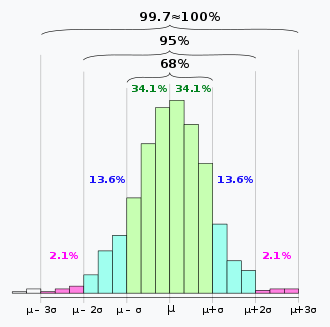
\includegraphics[width=0.8\linewidth]{pictures/68-95-99.7_RULE} \end{center}
\end{column}
\end{columns}
\end{frame}

\begin{frame}{Exercise 3}
\protect\hypertarget{exercise-3}{}
A population contains two million \textbf{zeros} an nine million
\textbf{ones}.

\begin{itemize}
\item
  \emph{Hint}: Make a table which contains all the possible values of
  the sample mean when \(n = 4\) and their probabilities.
\item
  \emph{Hint}: Remember that when the data is binary (\(0/1\)), there is
  a link between the sample mean and the sample proportion.
\end{itemize}

\begin{enumerate}
[(a)]
\setcounter{enumi}{1}
\tightlist
\item
  What is the approximate sampling distribution of the sample mean, when
  the sample size is \(n = 50\)?
\end{enumerate}
\end{frame}

\begin{frame}{(a) What is the sampling distribution of the sample mean,
when the sample size is \(n = 4\)?}
\protect\hypertarget{a-what-is-the-sampling-distribution-of-the-sample-mean-when-the-sample-size-is-n-4}{}
Drawing \(4\) observations from a population of zeros and ones, we have
\(5\) different possible samples

\begin{itemize}
\tightlist
\item
  \(\{0,0,0,0\}\) \(\rightarrow\) sample mean \(=0\)
\item
  \(\{1,0,0,0\}\) \(\rightarrow\) sample mean \(=1/4\)
\item
  \(\{1,1,0,0\}\) \(\rightarrow\) sample mean \(=1/2\)
\item
  \(\{1,1,1,0\}\) \(\rightarrow\) sample mean \(=3/4\)
\item
  \(\{1,1,1,1\}\) \(\rightarrow\) sample mean \(=1\)
\end{itemize}

\vspace{3mm}

\pause

\begin{itemize}
\tightlist
\item
  \(\color{blue}{\{Y_1,Y_2,Y_3,Y_4\} \mid Y_i = 0 \text{ or } Y_i = 1}\)\\
  sample mean
  \(= \frac{\sum_{i=1}^4Y_i}{4} = \frac{\text{number of 1s}}{\text{sample size}} =\)
  sample proportion \(=\hat{p}\).
\end{itemize}
\end{frame}

\begin{frame}{(a) What is the sampling distribution of the sample mean,
when the sample size is \(n = 4\)?}
\protect\hypertarget{a-what-is-the-sampling-distribution-of-the-sample-mean-when-the-sample-size-is-n-4-1}{}
\small

Formula for the probability of \(x\) successes in \(n\) trials
\href{https://en.wikipedia.org/wiki/Binomial_distribution}{\(\left[\text{Binomial distribution}\right]\)}

\[
P(x) ={\color{green}{\frac{n!}{x!\,(n-x)!}}}\,{\color{red}{p^x(1-p)^{n-x}}}, \quad \text{ for } {x = 1,\ldots,n}
\]

\begin{itemize}
\item
  Probability that the first \(x\) trials to be successes and the
  remaining \(n-x\) to be failures \[
  \color{red}{p\times p \times \ldots \times p \times (1-p)\times (1-p)\times \ldots \times (1-p) = p^x(1-p)^{n-x}}
  \]
\item
  The number of ways of arranging \(x\) successes in \(n\) trials is
  equal to the number of ways of choosing \(x\) objects from \(n\)
  objects \[
  \color{green}{{n \choose x} = \frac{n!}{x!\,(n-x)!}}
  \]
\end{itemize}
\end{frame}

\begin{frame}{(a) When \(n = 4\); \(x = 0,1,2,3,4\); \(p=9/11\)}
\protect\hypertarget{a-when-n-4-x-01234-p911}{}
\begin{columns}[T]
\begin{column}{0.48\textwidth}
\begin{table}
\centering
\begin{tabular}[t]{ccc}
\toprule
x & P(x) & p\_hat\\
\midrule
0 & 0.0011 & 0\\
1 & 0.0197 & 1/4\\
2 & 0.1328 & 1/2\\
3 & 0.3983 & 3/4\\
4 & 0.4481 & 1\\
\bottomrule
\end{tabular}
\end{table}
\end{column}

\begin{column}{0.48\textwidth}
\begin{center}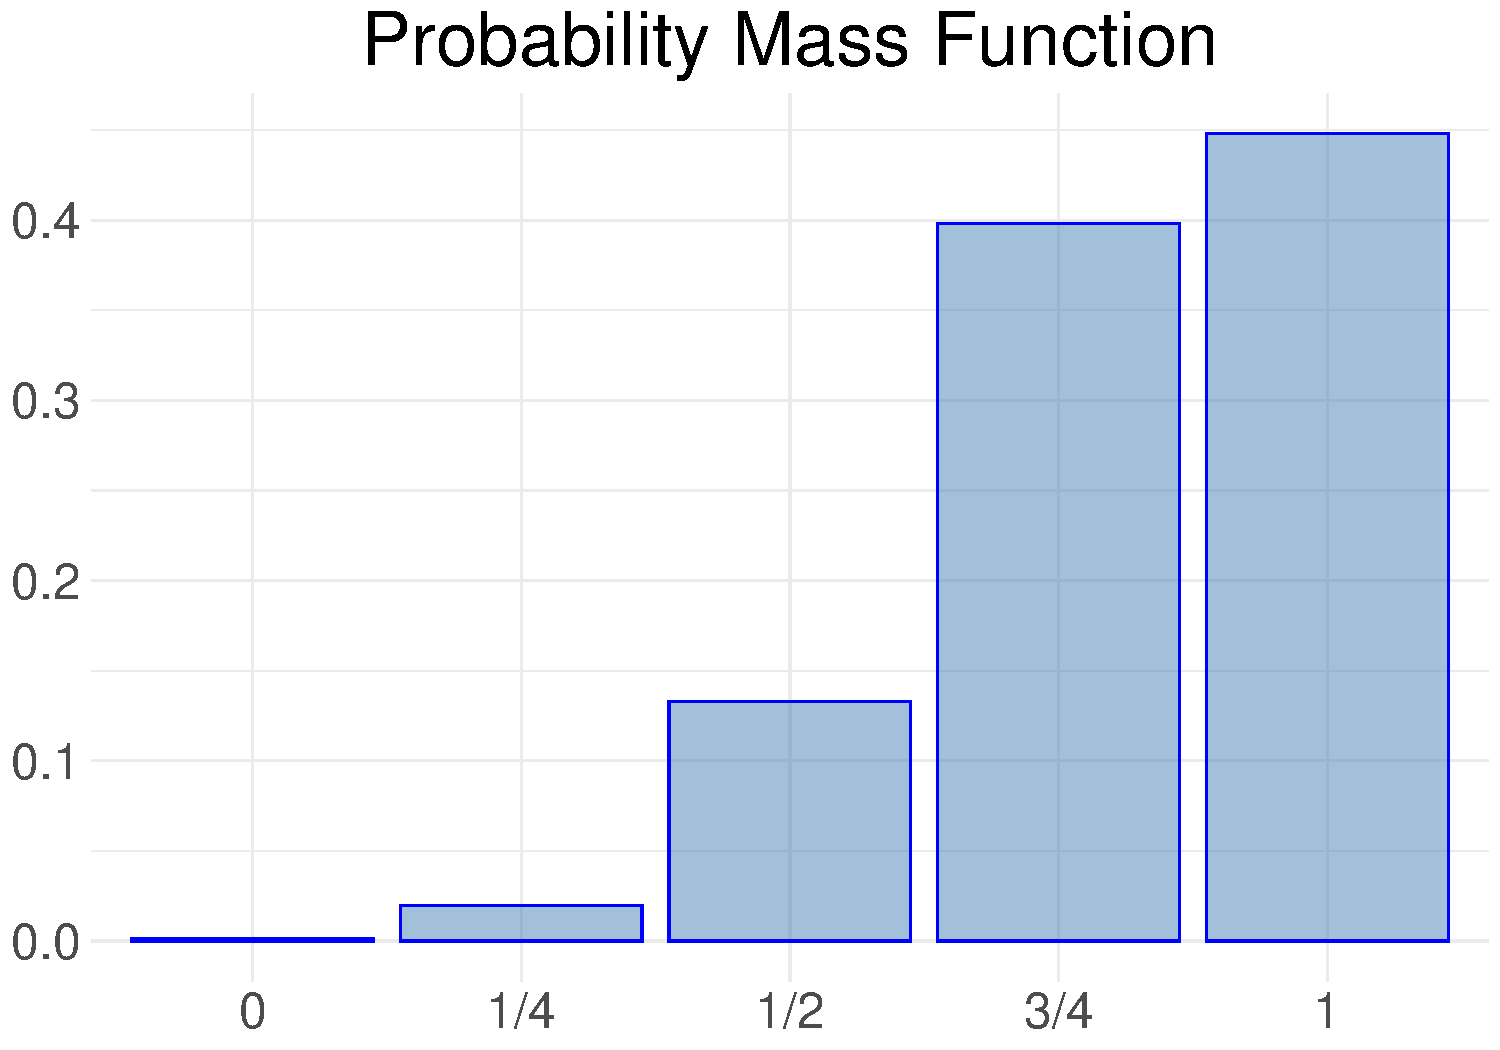
\includegraphics[width=0.9\linewidth]{ECON1013_Tutorial2_files/figure-beamer/unnamed-chunk-13-1} \end{center}
\end{column}
\end{columns}
\end{frame}

\begin{frame}{(b) What is the sampling distribution of the sample mean,
when the sample size is \(n = 50\)?}
\protect\hypertarget{b-what-is-the-sampling-distribution-of-the-sample-mean-when-the-sample-size-is-n-50}{}
\begin{itemize}
\item
  Formula for the probability of \(x\) successes in \(n\) trials \small
  \[
  P(x) ={\color{green}{\frac{n!}{x!\,(n-x)!}}}\,{\color{red}{p^x(1-p)^{n-x}}}, \quad \text{ for } {x = 1,\ldots,n}
  \]
\item
  Making table is complicated! \small
\end{itemize}

\begin{table}
\centering
\begin{tabular}{ccc}
\hline
x & P(x) & p\_hat \tabularnewline
\hline
0 & $\ldots$ & 0 \tabularnewline
1 & $\ldots$ & 1/50\tabularnewline
2 & $\ldots$ & 2/50 \tabularnewline
$\vdots$ & $\vdots$ & $\vdots$ \tabularnewline
50 & $\ldots$ & 50/50 \tabularnewline
\hline
\end{tabular}
\end{table}
\end{frame}

\begin{frame}{(b) When \(n = 50\); \(x = 0,1,\ldots,50\); \(p=9/11\)}
\protect\hypertarget{b-when-n-50-x-01ldots50-p911}{}
\begin{center}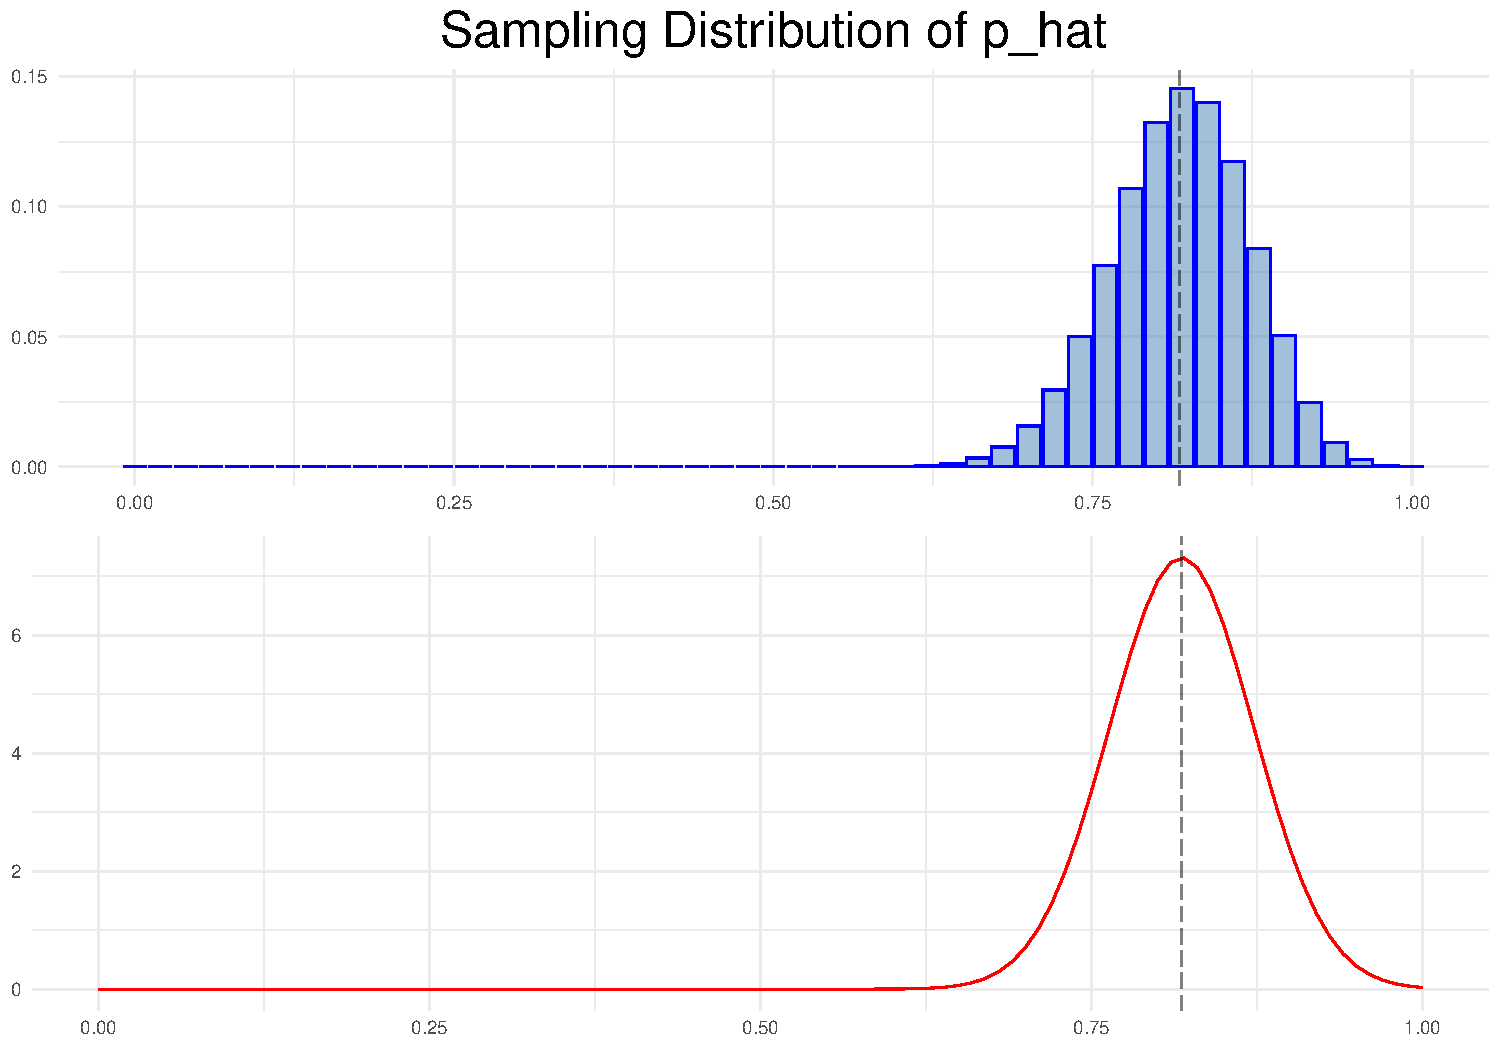
\includegraphics[width=0.9\linewidth]{ECON1013_Tutorial2_files/figure-beamer/unnamed-chunk-14-1} \end{center}
\end{frame}

\begin{frame}{Remark: Normal approximation for Binomial distribution}
\protect\hypertarget{remark-normal-approximation-for-binomial-distribution}{}
\begin{itemize}
\tightlist
\item
  Verify that \(n\) is large is enough \[
  n \cdot p \cdot (1-p) > 5,
  \] which is correct as \(50 \cdot (9/11) \cdot (2/11) \approx 7.44\).
\end{itemize}

\vspace{3mm}

\begin{itemize}
\tightlist
\item
  Hence, asymptotically, \[
  \hat{p} \sim \mathcal{N} \left({\color{red}{p}}, {\color{green}{\frac{p(1-p)}{n}}} \right)
  \] where \(\mu_{\hat{p}} = p = 9/11\),\\
  and
  \(\sigma_{\hat{p}} = \sqrt{\frac{p(1-p)}{n}} = \sqrt{\frac{(9/11)\cdot (2/11)}{50}} \approx 0.055\).
\end{itemize}
\end{frame}

\begin{frame}{Exercise 4}
\protect\hypertarget{exercise-4}{}
A small company has six employees, whose years of experience are \[
\left\{2\quad  4\quad  6\quad 6\quad 7\quad  8\right\}.
\] Two of these employees are to be chosen randomly for a particular
work group.

Let us consider the average number of years of experience of the two
employees \(\{X_1,X_2\}\) chosen randomly from the population of six. We
denote by \(\bar{X}_2\) the random variable sample means and by
\(\bar{x}_2\) its realization.
\end{frame}

\begin{frame}{Exercise 4}
\protect\hypertarget{exercise-4-1}{}
\begin{enumerate}
[(a)]
\item
  Compute the population mean \(\mu_X\) and the population variance
  \(\sigma_X^2\).
\item
  Compute the sampling distribution of \(\bar{X}_2\).
\item
  Compute the expectation of \(\bar{X}_2\) using the above sampling
  distribution and compare it with \(\mu_X\).
\item
  Compute the variance of \(\bar{X}_2\) using the sampling distribution
  computed above. Compare your result with \(\sigma^2_X/2\), which would
  compute the variance of \(\bar{X}_2\) if \(\{X_1,X_2\}\) was a simple
  random sample.
\end{enumerate}
\end{frame}

\begin{frame}{Exercise 4}
\protect\hypertarget{exercise-4-2}{}
The variance \(\sigma^2_X\) is unknown. Let us consider the sample
variance of the \(\{X_1,X_2\}\), denoted by \(s^2_2\).

\begin{enumerate}
[(a)]
\setcounter{enumi}{4}
\item
  Compute the sampling distribution of \(s^2_2\).
\item
  Compute the expectation of \(s^2_2\) using the above sampling
  distribution and compare it with \(\sigma^2_X\).
\item
  Verify that \(E(s^2_2)=N\sigma^2/(N-1)\), where \(N=6\).
\end{enumerate}

\emph{See also Tables 6.1 and 6.2 in the Textbook, and Exercise 6.56}
\end{frame}

\begin{frame}{Exercise 4}
\protect\hypertarget{exercise-4-3}{}
The problem suggests that the sampling is without replacement (the work
group should be formed by two persons). There are different 15 work
groups, with ages \[
\begin{array}{c|cccccc}
&2 & 4 & 6 & 6&7 & 8\\ \hline
2  & -- & (2,4) & (2,6) & (2,6) & (2,7) &(2,8)\\
 4  &-- &--  & (4,6) & (4,6) & (4,7) &(4,8)\\
 \vdots  &-- &--  & -- & \ddots & \cdots &\vdots 
\end{array} 
\] We consider only the element above the main diagonal, because the
matrix is symmetric and on the main diagonal we would have work groups
made of one person.
\end{frame}

\begin{frame}{(a) Compute the population mean \(\mu_X\) and the
population variance \(\sigma_X^2\).}
\protect\hypertarget{a-compute-the-population-mean-mu_x-and-the-population-variance-sigma_x2.}{}
\[\mu_X=\frac{2+4+6+6+7+8}{6}=5.5\] and
\[\sigma^2_X=\frac{(2-\mu_X)^2+\cdots (8-\mu_x)^2}{6}=23.5/6=3.916667.\].
\end{frame}

\begin{frame}{(b) Compute the sampling distribution of \(\bar{X}_2\).}
\protect\hypertarget{b-compute-the-sampling-distribution-of-barx_2.}{}
\[
\begin{array}{c|ccccccccc}
\bar{x}_2 & 3 & 4 & 4.5 & 5&  5.5 & 6 & 6.5 & 7& 7.5\\\hline
p(\bar{x}_2) & 1/15 & 2/15 & 1/15 & 3/15 & 1/15 & 2/15 & 2/15 & 2/15 & 1/15
\end{array}
\]
\end{frame}

\begin{frame}{(c) Compute the expectation of \(\bar{X}_2\) using the
above sampling distribution and compare it with \(\mu_X\).}
\protect\hypertarget{c-compute-the-expectation-of-barx_2-using-the-above-sampling-distribution-and-compare-it-with-mu_x.}{}
\[
\sum_{j=1}^9 \bar{x}_{2,j}p(\bar{x}_{2,j})=5.5
\]

\begin{itemize}
\tightlist
\item
  The estimator is unbiased.
\end{itemize}
\end{frame}

\begin{frame}{(d) Compute the variance of \(\bar{X}_2\) using the
sampling distribution computed above. Compare your result with
\(\sigma^2_X/2\), which would compute the variance of \(\bar{X}_2\) if
\(\{X_1,X_2\}\) was a simple random sample.}
\protect\hypertarget{d-compute-the-variance-of-barx_2-using-the-sampling-distribution-computed-above.-compare-your-result-with-sigma2_x2-which-would-compute-the-variance-of-barx_2-if-x_1x_2-was-a-simple-random-sample.}{}
\[
\sum_{j=1}^9 (\bar{x}_{2,j}-\mu_X)^2p(\bar{x}_{2,j})=\frac{23.5}{15}=1.566667
\]

\begin{itemize}
\tightlist
\item
  Note that we should not apply the formula \(\sigma^2_X/2=23.5/12\) but
  we should apply the finite population correction factor. \[
  \frac{\sigma^2_X}{2}\frac{N-n}{N-1}=\frac{23.5}{12}\frac{4}{5}=\frac{23.5}{15}
  \]
\end{itemize}
\end{frame}

\begin{frame}{(e) Compute the sampling distribution of \(s^2_2\).}
\protect\hypertarget{e-compute-the-sampling-distribution-of-s2_2.}{}
\[
\begin{array}{c|ccccccc}
s^2_2 
& 0.0 &   0.5  &  2.0 & 4.5  &  8 & 12.5 &  18\\ \hline
p(s^2_2) & 1/15 & 3/15 & 5/15 &  1/15 & 3/15 & 1/15 & 1/15
\end{array}
\]
\end{frame}

\begin{frame}{(f) Compute the expectation of \(s^2_2\) using the above
sampling distribution and compare it with \(\sigma^2_X\).}
\protect\hypertarget{f-compute-the-expectation-of-s2_2-using-the-above-sampling-distribution-and-compare-it-with-sigma2_x.}{}
\[
\sum_{j=1}^7 s^2_{2,j}p(s^2_{2,j})=5.5
\]

\begin{itemize}
\tightlist
\item
  The estimator is biased.
\end{itemize}
\end{frame}

\begin{frame}{(g) Verify that \(E(s^2_2)=N\sigma^2/(N-1)\), where
\(N=6\).}
\protect\hypertarget{g-verify-that-es2_2nsigma2n-1-where-n6.}{}
Multiplying the number above by \(5/6\) we get \(\sigma^2_X\).
\end{frame}

\end{document}
